%=======================================================================
% DROP-IN REPLACEMENT for \subsection{Power-to-heat-to-power cycle analysis}
% It closes the three \todo{} blocks in that subsection.
%
% Numbers: boreas.py v1.3, reference case of Table~\ref{tab:conditions},
% n_s = 99, generated 2026-10-25. Tables are machine-generated by
% src/mktex.py from papercalc.json -- regenerate rather than hand-edit.
%
% Requires: \etaORC, \COP (already in the paper); siunitx; graphicx.
% New label targets: tab:states, tab:cycles, tab:UA, tab:T3e,
%                    fig:ts, fig:composite, fig:composite-stores.
%=======================================================================
\subsection{Power-to-heat-to-power cycle analysis}
\label{sec:res-cycles}

The plant models are those of the hairpin study and are unchanged here. The
store reaches them through a single quantity, the realized water outlet
$\overline{T}_\mathrm{2d}$, which sets the ORC evaporating temperature
$T_\mathrm{3e}$; everything else in Figure~\ref{fig:ts} and
Tables~\ref{tab:states} and \ref{tab:cycles} is independent of the borehole.
Stating that interface explicitly matters for the parametric work of
Section~\ref{sec:res-param}: the geothermal source temperature moves the
$\COP$ and leaves the ORC untouched, while the cascade specification moves
$\overline{T}_\mathrm{2d}$ and therefore the ORC alone.

\begin{figure}[htbp]
\centering
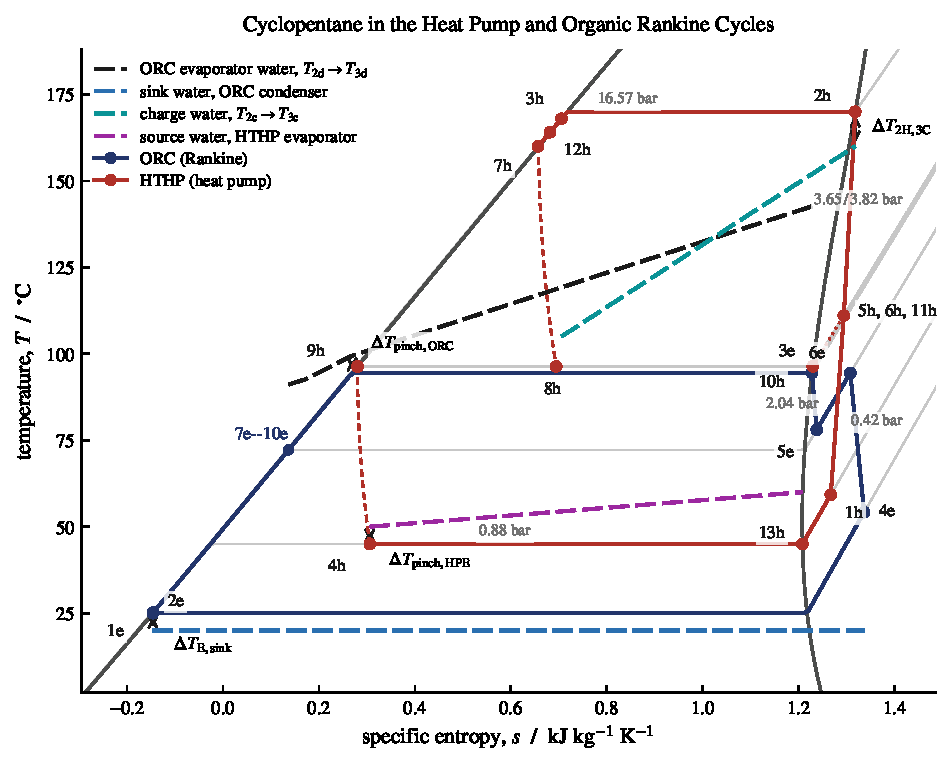
\includegraphics[width=\linewidth]{figures/BOREAS_Ts_combined_water.pdf}
\caption{The two cycles on one $T$--$s$ diagram at the reference case, with
the four water streams. Water cannot be drawn on these axes directly, since
its entropy is on an unrelated scale; what is plotted is the water
temperature at each point of the exchanger, placed at the entropy the working
fluid has at that same point, the two being tied together by cumulative duty.
The vertical gap is therefore the local approach at every abscissa and the
pinch is its narrowest point. The construction is a duty mapping, not a
thermodynamic path, and the abscissa carries no meaning for the water itself.}
\label{fig:ts}
\end{figure}

% Generated from boreas.py v1.3, reference case = 1000-well vertical
% array in double rows on four islands. Do not hand-edit: regenerate
% with mktex.py so the table cannot drift from the model.
\begin{table}[htbp]
\centering
\caption{\emph{Supplementary material.} State points of the two cycles at the reference case. The ORC is a double-stage reheat cycle with a regenerator (7e--10e); the HTHP is a two-stage flash-economizer cycle, in which 7h throttles into a drum at $p_\mathrm{int}$, the saturated liquid 9h throttles on to 4h and the flash vapour 10h rejoins the second stage. States 5h, 6h and 11h coincide.}
\label{tab:states}
\small
\begin{tabular}{@{}l r r r r | l r r r r@{}}
\toprule
ORC & $T$ [\si{\celsius}] & $p$ [\si{\bar}] & $h$ [\si{\kilo\joule\per\kilogram}] & $s$ [\si{\kilo\joule\per\kilogram\per\kelvin}] & HTHP & $T$ [\si{\celsius}] & $p$ [\si{\bar}] & $h$ & $s$ \\
\midrule
1e & 25.00 & 0.423 & -45.43 & -0.1462 & 1h & 59.25 & 0.879 & 403.50 & 1.2672 \\
2e & 25.14 & 3.647 & -44.92 & -0.1459 & 2h & 170.00 & 16.575 & 543.38 & 1.3183 \\
3e & 94.46 & 3.647 & 445.68 & 1.2279 & 3h & 168.00 & 16.575 & 271.94 & 0.7058 \\
4e & 54.19 & 0.423 & 398.44 & 1.3368 & 4h & 45.00 & 0.879 & 97.37 & 0.3063 \\
5e & 78.06 & 2.035 & 426.11 & 1.2378 & 5h & 111.05 & 3.818 & 472.51 & 1.2943 \\
6e & 94.46 & 2.035 & 451.33 & 1.3079 & 6h & 111.05 & 3.818 & 472.51 & 1.2943 \\
7e & 72.20 & 2.035 & 45.89 & 0.1370 & 7h & 159.96 & 16.575 & 250.46 & 0.6566 \\
8e & 72.28 & 3.647 & 46.16 & 0.1371 & 8h & 96.34 & 3.818 & 250.46 & 0.6946 \\
9e & 72.20 & 3.647 & 45.99 & 0.1366 & 9h & 96.34 & 3.818 & 97.37 & 0.2803 \\
10e & 72.22 & 3.647 & 46.02 & 0.1367 & 10h & 96.34 & 3.818 & 448.11 & 1.2296 \\
 & & & &  & 11h & 111.05 & 3.818 & 472.51 & 1.2943 \\
 & & & &  & 12h & 164.04 & 16.575 & 261.29 & 0.6815 \\
 & & & &  & 13h & 45.00 & 0.879 & 384.28 & 1.2081 \\
\bottomrule
\end{tabular}
\end{table}

\begin{table}[htbp]
\centering
\caption{Cycle indicators at the reference case. The plant models are those of the hairpin study; only $T_\mathrm{3e}$, which follows the realized outlet $\overline{T}_\mathrm{2d}$, depends on the store. Electrical input to the heat pump is \SI{3045.9}{\kilo\watt} and the charging water flow \SI{30.48}{\kilogram\per\second}; per fin tube the store sees \SI{0.5307} and \SI{0.5340}{\kilogram\per\second} on charge and discharge.}
\label{tab:cycles}
\small
\begin{tabular}{@{}l r r@{}}
\toprule
quantity & ORC & HTHP \\
\midrule
$\etaORC$ & 0.1471 & -- \\
$\COP$ & -- & 2.4731 \\
$y$, reheat mass fraction & 0.8070 & -- \\
$x_\mathrm{8h}$, flash vapour fraction & -- & 0.4365 \\
$\varepsilon_\mathrm{R1}$ & -- & 0.2053 \\
$\varepsilon_\mathrm{R2}$ & -- & 0.1197 \\
$p_\mathrm{evap}$ [\si{\bar}] & 3.647 & 0.879 \\
$p_\mathrm{int}$ [\si{\bar}] & 2.035 & 3.818 \\
$p_\mathrm{cond}$ [\si{\bar}] & 0.423 & 16.575 \\
$T_\mathrm{3e}$ [\si{\celsius}] (pinch-limited) & 94.46 & -- \\
evaporator pinch [\si{\kelvin}] & 5.00 & -- \\
duty [\si{\kilo\watt}], field & 7156.2 & 7156.2 \\
\bottomrule
\end{tabular}
\end{table}


\paragraph{The evaporator pinch is interior, and the hot-end rule is not
merely optimistic} Figure~\ref{fig:composite} gives the composite curves of
the ORC evaporator. The water glides down from $\overline{T}_\mathrm{2d}$ as
a nearly straight sensible line while the working fluid preheats and then
goes flat at $T_\mathrm{3e}$ for the remaining four fifths of the duty, so
the smallest approach falls neither at the hot end nor at the cold end but at
the corner where boiling begins, at \SI{16}{\percent} of the load. The
approach is \SI{18}{\kelvin} at the cold end and \SI{51}{\kelvin} at the hot
end, and \SI{5}{\kelvin} in between.

The consequence is stronger than a loss of accuracy. The cold composite that
a hot-end approach rule alone would permit,
$T_\mathrm{3e}=\overline{T}_\mathrm{2d}-\Delta T_\mathrm{2D,3E}$, is drawn
dashed in Figure~\ref{fig:composite}(a): it lies \emph{above} the water curve
over \SI{78}{\percent} of the duty. That is not a slightly optimistic design
but a violation of the second law, and the efficiency computed from it is
unreachable at any size of exchanger. Writing $T_\mathrm{3e}$ as the minimum
of the two constraints is therefore not a refinement of the hot-end rule; in
this plant the hot-end rule never binds at all, at any storage temperature in
the range examined in Section~\ref{sec:res-param}, and it is retained only
because it would bind in a plant with a smaller water glide.

\begin{figure}[htbp]
\centering
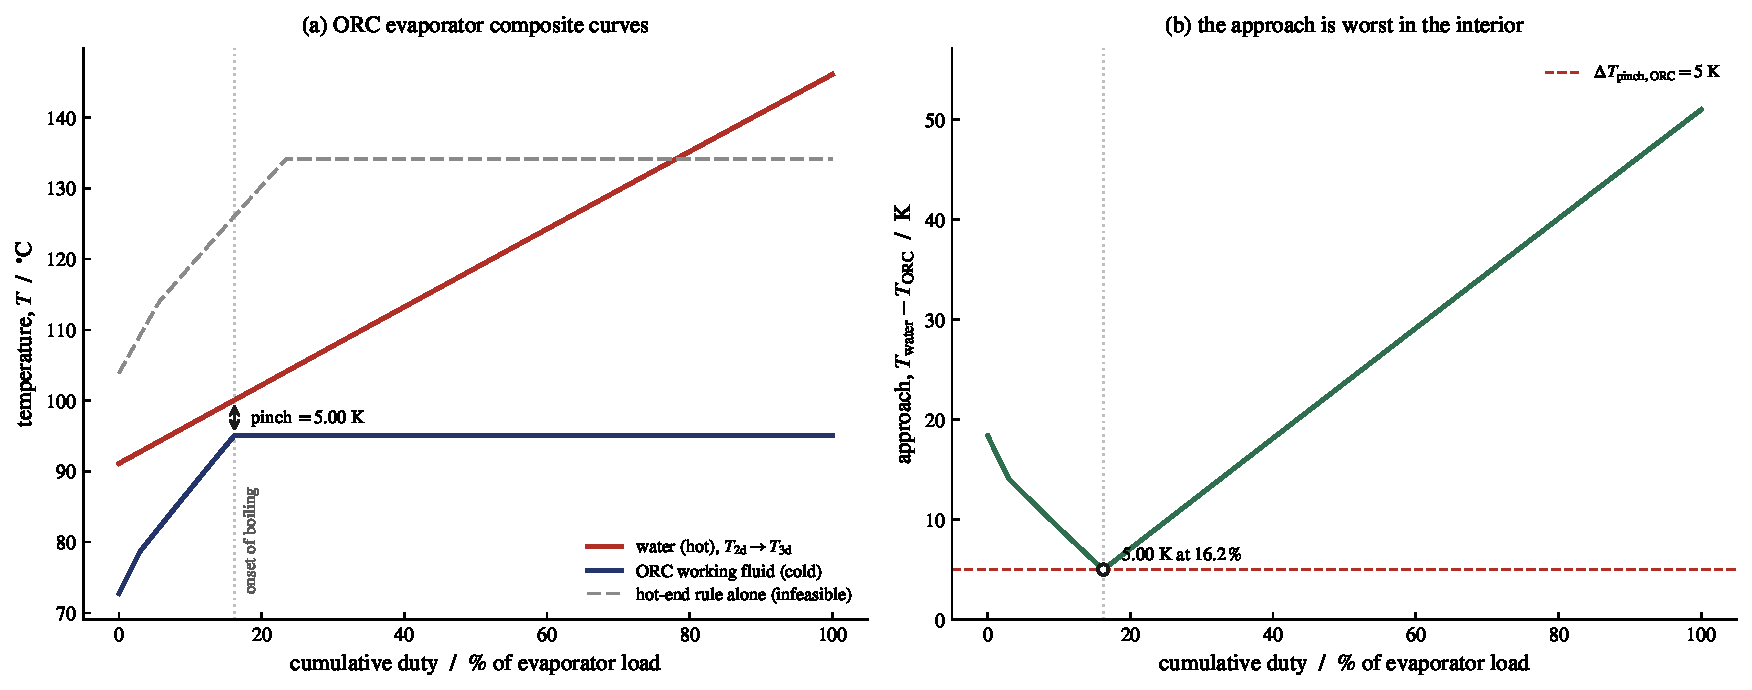
\includegraphics[width=\linewidth]{figures/BOREAS_ORC_composite.pdf}
\caption{ORC evaporator composite curves at the reference case (a) and the
approach profile along the exchanger (b). The pinch sits at the onset of
boiling, at \SI{16}{\percent} of the duty. The dashed grey curve in (a) is
the cold composite that the hot-end approach rule alone would permit; it
crosses the water curve and runs backwards over \SI{78}{\percent} of the
load. Both streams follow real enthalpy, so the latent plateau is flat rather
than smeared into a straight line in temperature.}
\label{fig:composite}
\end{figure}

\paragraph{How the loss to the formation reaches the cycle}
Figure~\ref{fig:composite-stores} and Table~\ref{tab:T3e} trace the chain
from the store to the ORC. Loss to the formation lowers
$\overline{T}_\mathrm{2d}$; the water line flattens and drops; the
pinch-limited $T_\mathrm{3e}$ follows it down; and $\etaORC$ follows that. At
the reference case the vertical array gives up
\SI{3.2}{\kelvin} of $\overline{T}_\mathrm{2d}$ against the adiabatic limit
and \SI{0.57}{\kelvin} of $T_\mathrm{3e}$, which is \SI{0.6}{\percent} of
$\etaORC$; the isolated well gives up \SI{41.8}{\kelvin} and
\SI{7.0}{\kelvin}, or \SI{7.5}{\percent} of $\etaORC$. The cycle penalty is
thus small beside the storage penalty itself, and the round-trip efficiency
is reduced approximately in proportion to $\eta_\mathrm{storage}$, as
Section~\ref{sec:res-formation} records; the ORC term is the second-order
correction that makes the proportionality inexact.

\begin{figure}[htbp]
\centering
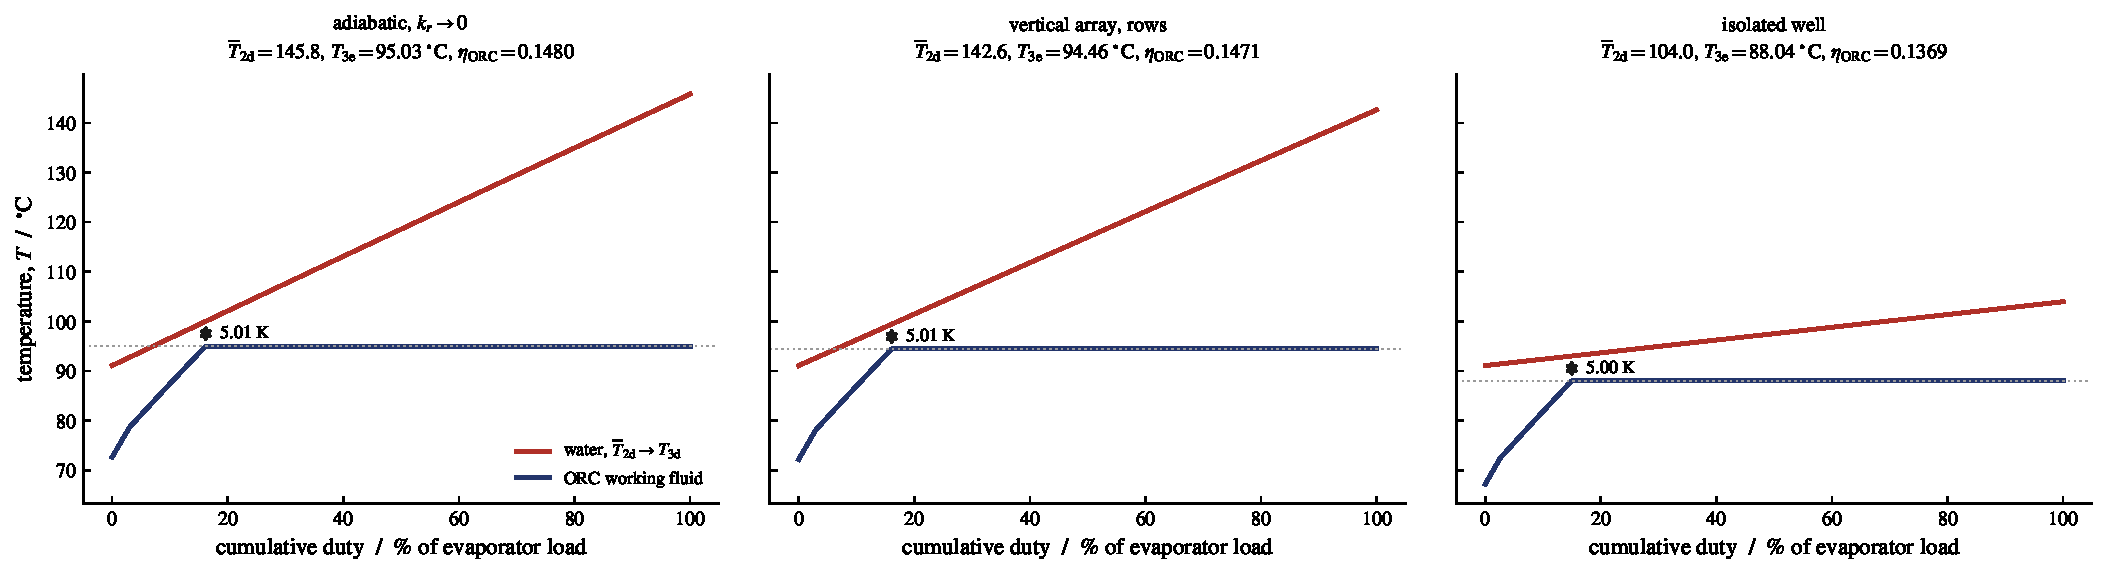
\includegraphics[width=\linewidth]{figures/BOREAS_ORC_composite_stores.pdf}
\caption{ORC evaporator composites for three stores on a common axis. The
pinch is held at \SI{5}{\kelvin} in each case by construction, so what moves
is the whole water line and with it $T_\mathrm{3e}$. For the isolated well
the water arrives at \SI{104.0}{\celsius} and glides only
\SI{13}{\kelvin}, because the store cannot deliver its design duty.}
\label{fig:composite-stores}
\end{figure}

\paragraph{What the approach temperatures cost} Table~\ref{tab:UA} gives the
conductance each exchanger requires, integrated over the same composite
curves. Reporting it closes a gap that would otherwise make every approach
temperature a free parameter: tightening $\Delta T_\mathrm{pinch,ORC}$ raises
$\etaORC$ with nothing to pay for it unless $UA$ is carried alongside. The
four exchangers require \SI{2297}{\kilo\watt\per\kelvin} in total for the
reference field. The HTHP condenser is the least conductance-hungry
(\SI{245}{\kilo\watt\per\kelvin}) because its \SI{55}{\kelvin} water glide is
matched against a long desuperheating section, and the ORC condenser the most
(\SI{1152}{\kilo\watt\per\kelvin}) because a \SI{5}{\kelvin} approach against
an isothermal sink is expensive by construction.

\begin{table}[htbp]
\centering
\caption{Conductance required by the four plant exchangers at the reference case, integrated over the real composite curves. $\Delta T_\mathrm{eff}=\dot Q/UA$ is the approach that reproduces the conductance; with a phase change on one side it is the correct generalization of the log-mean difference, which the LMTD is not. The recovered pinches reproduce the specified approaches exactly, which is the check on the construction.}
\label{tab:UA}
\small
\begin{tabular}{@{}l r r r r@{}}
\toprule
exchanger & $\dot Q$ [\si{\kilo\watt}] & $UA$ [\si{\kilo\watt\per\kelvin}] & $\Delta T_\mathrm{eff}$ [\si{\kelvin}] & pinch [\si{\kelvin}] \\
\midrule
orc evaporator & 7156.2 & 433.0 & 16.53 & 5.01 \\
orc condenser & 6103.6 & 1151.5 & 5.30 & 5.00 \\
hthp condenser & 7156.2 & 244.6 & 29.26 & 10.00 \\
hthp evaporator & 4262.6 & 468.3 & 9.10 & 5.00 \\
\midrule
total & 24678.6 & 2297.3 & -- & 5.00 \\
\bottomrule
\end{tabular}
\end{table}

\begin{table}[htbp]
\centering
\caption{The store reaches the ORC through one number. Loss to the formation lowers the realized water outlet $\overline{T}_\mathrm{2d}$, the pinch-limited evaporating temperature follows and $\etaORC$ with it.}
\label{tab:T3e}
\small
\begin{tabular}{@{}l r r r@{}}
\toprule
store & $\overline{T}_\mathrm{2d}$ [\si{\celsius}] & $T_\mathrm{3e}$ [\si{\celsius}] & $\etaORC$ \\
\midrule
adiabatic, $k_r\to0$ & 145.79 & 95.03 & 0.1480 \\
vertical array, 1000 wells, rows & 142.62 & 94.46 & 0.1471 \\
fan, 1000 wells, rows & 115.85 & 89.90 & 0.1400 \\
isolated well & 103.97 & 88.04 & 0.1369 \\
\bottomrule
\end{tabular}
\end{table}

